% G2-6 Grid Search dan Random Search pada dua parameter.
% Sumber: diadaptasi dari bergstra2012 (Gambar 1, hlm. 284).
% Titik acak ditulis sebagai koordinat tetap (tidak dibangkitkan saat compile).
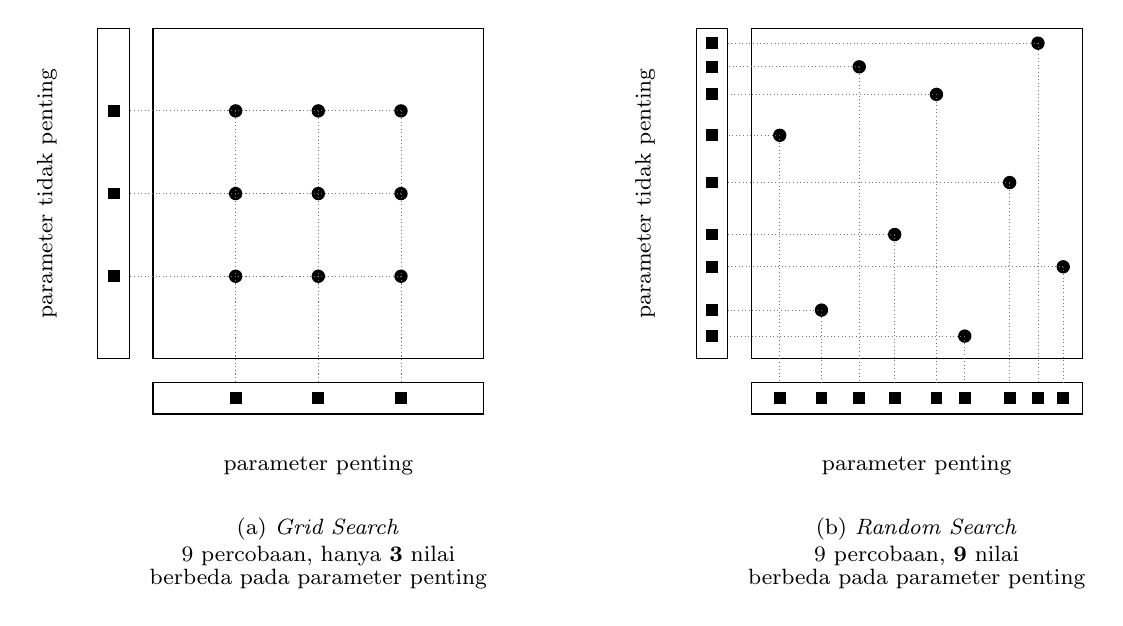
\begin{tikzpicture}[x=1mm,y=1mm,font=\footnotesize,
    titik/.style={fill=black,circle,inner sep=0pt,minimum size=1.7mm},
    proy/.style={draw,black!55,densely dotted,line width=0.3pt},
    tik/.style={fill=black,rectangle,inner sep=0pt,minimum size=1.5mm}]

  % ===================== panel (a) Grid Search =====================
  \begin{scope}
    \draw (0,0) rectangle (42,42);
    % sumbu
    \node[rotate=90,anchor=south] at (-11,21) {parameter tidak penting};
    \node[anchor=north] at (21,-11) {parameter penting};
    % pita proyeksi
    \draw (0,-7) rectangle (42,-3);
    \draw (-7,0) rectangle (-3,42);

    % 9 titik grid 3x3
    \foreach \x in {10.5,21,31.5}{
      \foreach \y in {10.5,21,31.5}{
        \node[titik] at (\x,\y) {};
        \draw[proy] (\x,\y) -- (\x,-3);
        \draw[proy] (\x,\y) -- (-3,\y);
      }}
    % proyeksi: hanya 3 nilai berbeda di tiap sumbu
    \foreach \x in {10.5,21,31.5}{\node[tik] at (\x,-5) {};}
    \foreach \y in {10.5,21,31.5}{\node[tik] at (-5,\y) {};}

    \node[anchor=north,align=center] at (21,-19)
      {(a) \textit{Grid Search}\\9 percobaan, hanya \textbf{3} nilai\\[-1pt]
       berbeda pada parameter penting};
  \end{scope}

  % ===================== panel (b) Random Search =====================
  \begin{scope}[xshift=76mm]
    \draw (0,0) rectangle (42,42);
    \node[rotate=90,anchor=south] at (-11,21) {parameter tidak penting};
    \node[anchor=north] at (21,-11) {parameter penting};
    \draw (0,-7) rectangle (42,-3);
    \draw (-7,0) rectangle (-3,42);

    % 9 titik acak, koordinat tetap
    \foreach \x/\y in {3.6/28.4, 8.9/6.2, 13.7/37.1, 18.2/15.8, 23.5/33.6,
                       27.1/2.9, 32.8/22.4, 36.4/40.1, 39.6/11.7}{
      \node[titik] at (\x,\y) {};
      \draw[proy] (\x,\y) -- (\x,-3);
      \draw[proy] (\x,\y) -- (-3,\y);
      \node[tik] at (\x,-5) {};
      \node[tik] at (-5,\y) {};
    }

    \node[anchor=north,align=center] at (21,-19)
      {(b) \textit{Random Search}\\9 percobaan, \textbf{9} nilai\\[-1pt]
       berbeda pada parameter penting};
  \end{scope}

\end{tikzpicture}
